\documentclass{article}
\usepackage{gvv-book}
\usepackage{gvv}
\usepackage{amsmath}
\usepackage{amsfonts}
\usepackage{tikz}
\usepackage{setspace}
\usepackage{gensymb}
\singlespacing
\usepackage[cmex10]{amsmath}
\usepackage{amsthm}
\usepackage{mathrsfs}
\usepackage{txfonts}
\usepackage{stfloats}
\usepackage{bm}
\usepackage{cite}
\usepackage{cases}
\usepackage{subfig}
\usepackage{longtable}
\usepackage{multirow}
\usepackage{enumitem}
\usepackage{mathtools}
\usepackage{tikz}
\usepackage{circuitikz}
\usepackage{verbatim}
\usepackage[breaklinks=true]{hyperref}
\usepackage{tkz-euclide}
\usepackage{listings}
\usepackage{color}    
\usepackage{array}    
\usepackage{longtable}
\usepackage{calc}     
\usepackage{multirow} 
\usepackage{hhline}   
\usepackage{ifthen}   
\usepackage{lscape}     
\usepackage{chngcntr}
\usepackage{graphicx}
\usepackage{float}
\usepackage{multicol}
\usepackage[a4paper, left=3.5cm, right=3.5cm]{geometry}





\begin{document}
\title{
ASSIGNMENT 1: GATE 2007 \\
    AE : AEROSPACE ENGINEERING }
\author{AI25BTECH11029 - Samyak Gondane }
\maketitle


\begin{center}
    \textbf{Read the following instructions carefully}
\end{center}
\begin{enumerate}
    \item This question paper contains 85 objective type questions. Q. 1 to Q. 20 carry \textbf{one} mark each and Q. 21 to Q. 85 carry \textbf{two} marks each.
    \item Attempt all the questions.
    \item Questions must be answered on \textbf{O}bjective \textbf{R}esponse \textbf{S}heet (\textbf{ORS}) by darkening the appropriate bubble (marked A, B, C, D) using HB pencil against the question number on the left hand side of the \textbf{ORS. Each question has only one correct answer.} In case you wish to change an answer, erase the old answer completely.
    \item Wrong answers will carry NEGATIVE marks. In Q.1 to Q.20, \textbf{0.25} marks will be deducted for each wrong answer. In Q.21 to Q.76, Q.78, Q.80, Q.82 and in Q.84, \textbf{0.5} marks will be deducted for each wrong answer. However, there is no negative marking in Q.77, Q.79, Q.81, Q.83 and in Q.85. More than one answer bubbled against a question will be taken as an incorrect response. Unattempted questions  will not carry any marks.
    \item Write your registration number, your name and nae of the examination centre at the specified locations on the right half of the \textbf{ORS.}
    \item Using HB pencil, darken the appropriate bubble under each digit of your registration number and the letters corresponding to your paper code.
    \item Calculator is allowed in the examination hall.
    \item Charts, graph sheets or tables are NOT allowed in the examination hall.
    \item Rough work can be done on the question paper itself. Additionally blank pages are given at the end of the question paper for rough work.
    \item This question paper contains \textbf{24} printed pages including pages for rough work. Please check all pages and report, if there is any discrepancy.
\end{enumerate}

\newpage

\begin{center}
    \textbf{Q. 1 - Q. 20 carry one mark each)}
\end{center}

\begin{enumerate}
    \item Which one of the following engines should be used by a subsonic passenger transport airplane for minimum specific fuel consumption?
    \begin{enumerate}
        \item Turbojet engine with afterburner
        \item Turbofan engine
        \item Ramjet engine
        \item Scramjet engine
    \end{enumerate}
    

    \item A spring-mass-damper system with a mass of $1 \, \mathrm{kg}$ is found to have a damping ratio of 0.2 and a natural frequency of $5 \, \mathrm{rad/s}$. The damping of the system is given by 
    \begin{multicols}{4}
    \begin{enumerate}
        \item $2 \, \mathrm{Ns/m}$ 
        \item $2 \, \mathrm{N/s}$ 
        \item $0.2 \, \mathrm{kg/s}$ 
        \item $0.2 \, \mathrm{N/m}$
    \end{enumerate}
    \end{multicols}
        

    \item If $f(\theta)$$ = \myvec{\cos\theta & \sin\theta \\
        -\sin\theta & \cos\theta}, \space then $f($\alpha$) f($\beta$) = 
    \begin{multicols}{2}
    \begin{enumerate}
        \item $f(\alpha/\beta)$ 
        \item $f(\alpha + \beta)$ 
        \item $f(\alpha - \beta)$ 
        \item $2 \times 2$ zero matrix
    \end{enumerate}
    \end{multicols}


    \item An artificial satellite remains in orbit and does not fall to the earth because
    \begin{enumerate}
        \item the centrifugal force acting on it balance the gravitational attraction 
        \item the on-board rocket motors provide continuous boost to keep it in orbit 
        \item its transverse velocity keeps it from hitting the earth although it falls  continuously 
        \item due to its high speed it derives sufficiant lift from the rarefied atmosphere 
    \end{enumerate}


    \item The Euler iteration formula for numerically integrating a first order nonlinear differential equation of form $x = f(x)$, with a constant step size of $\Delta t$ is 
    \begin{multicols}{2}
    \begin{enumerate}
        \item $x_{k+1} = x_k - \Delta t \times f(x_k)$ 
        \item $x_{k+1} = x_k + \left( \Delta t^2 / 2 \right) \times f(x_k)$ 
        \item $x_{k+1} = x_k - (1 / \Delta t) \times f(x_k)$ 
        \item $x_{k+1} = x_k + \Delta t \times f(x_k)$
    \end{enumerate}
    \end{multicols}
        

    \item The number of natural frequencies of an elastic beam with cantilever boundary conditions is
    \begin{multicols}{4}
    \begin{enumerate}
        \item 1 
        \item 3 
        \item 1000 
        \item Infinite
    \end{enumerate}
    \end{multicols}
        

    \item For maximum range of a glider, which of the following conditions is true?
    \begin{enumerate}
        \item Lift to drag ratio is maximum
        \item Rate of descent is minimum
        \item Descent angle is maximum
        \item Lift to weight ratio is maximum 
    \end{enumerate}
        
\newpage
    \item An airplane with a larger wing as compared to a smaller wing will necessarily have 
    \begin{enumerate}
        \item More longitudinal static stability
        \item Less longitudinal static stability
        \item Same longitudinal static stability
        \item More longitudinal static stability for an aft tail airplane if aerodynamic center of the larger wing is behind the center of gravity of the airplane
    \end{enumerate}
        

    \item The minimum value of$J(x) = x^2 - 7x + 30$ occurs at
    \begin{multicols}{2}
    \begin{enumerate}
        \item $x = 7/2$ 
        \item $x = 7/30$ 
        \item $x = 30/7$ 
        \item $x = 30$
    \end{enumerate}
    \end{multicols}
        

    \item Two airplanes are identical except for the location of the wing. The longitudinal static stability of the airplane with low wing configuration will be 
    \begin{enumerate}
        \item More than the airplane with high wing configuration
        \item less than the airplane with high wing configuration
        \item same as the airplane with high wing configuration
        \item more if elevator is deflected
    \end{enumerate}
        

    \item For a fixed centre of gravity location of an airplane, when the propeller is mounted on the nose of the fuselage 
    \begin{enumerate}
        \item longitude static stability increases
        \item longitude static stability decreases
        \item longitude static stability remains same
        \item longitude static stability is maximum
    \end{enumerate}
        

    \item Let an airplane in a steady level flight be trimmed at a certain spee(D) A level and steady flight at a higher speed could be achived by changing 
    \begin{enumerate}
        \item Engine throttle only
        \item Elevator only
        \item Throttle and elevator together
        \item Rudder only
    \end{enumerate}
        

    \item For a plane strain problem in the $x-y$ plane, in general, the non-zero stress terms are 
    \begin{multicols}{2}
    \begin{enumerate}
        \item $\sigma_{xx}, \sigma_{yy}, \sigma_{zz}, \sigma_{xy}$ 
        \item $\sigma_{xx}, \sigma_{yy}, \sigma_{xy}$ 
        \item $\sigma_{xx}, \sigma_{yy}, \sigma_{xy}, \sigma_{xz}$ 
        \item $\sigma_{xx}, \sigma_{yy}, \sigma_{xy}, \sigma_{zz}$
    \end{enumerate}
    \end{multicols}
        

    \item For an elastic anisotropic solid, the number of independent elastic constants in its constitutive equations is
    \begin{multicols}{4}
    \begin{enumerate}
        \item 2 
        \item 9 
        \item 21 
        \item 36
    \end{enumerate}
    \end{multicols}
        

    \item Total pressure at a point is defined as the pressure when the flow is brought to rest 
    \begin{enumerate}
        \item Adiabatically
        \item Isentropically
        \item Isothermally
        \item Isobarically
    \end{enumerate}
        

    \item The drag divergence Mach number of an airfoil 
    \begin{enumerate}
        \item Is a fixed number for a given airfoil
        \item Is always higher than the critical Mach number
        \item Is equal to the critical Mach number at zero angle of attack
        \item Is the Mach number at which a shock wave first appears on the airfoil
    \end{enumerate}
        

    \item On which one of the following thermodynamic cycles does an ideal ramjet operate? 
    \begin{enumerate}
        \item The Rankine cycle
        \item The Brayton cycle
        \item The Carnot cycle
        \item The Diesel cycle 
    \end{enumerate}
        

    \item Across a normal shock 
    \begin{enumerate}
        \item both temperature and total pressure decreases
        \item both temperature and total pressure remains constant
        \item total pressure remain constant but total temperature decreases
        \item total temperature remains constant but total pressure decreases
    \end{enumerate}
        

    \item The Joukowski airfoil is studied in aerodynamics because 
    \begin{enumerate}
        \item It is used in many aircraft
        \item It is easily transformed into a circle, mathematically
        \item It has a simple geometry
        \item It has the highest lift curve slope among all airfoils
    \end{enumerate}
        

    \item One of the criteria for high-speed airplanes is that the critical Mach number should be as high as possible. Therefore, high-speed subsonic airplanes are usually designed with 
    \begin{enumerate}
        \item Thick airfoils
        \item Thin airfoils
        \item Laminar flow airfoils
        \item Diamond airfoils
    \end{enumerate}
        

\newpage
\begin{center}
    \textbf{Q. 21 - Q. 75 carry two marks each}
\end{center}


    \item Two identical earth satellites $A$ and $B$ are in circular orbits at altitudes $h_A$ and $h_B$ above the earth's surface respectively, with $h_A > h_B$. If $E$ denotes the total mechanical energy, $T$ the kinetic energy and $V$ the gravitational potential energy of a satellite, then: 
    \begin{enumerate}
        \item $E_A > E_B$ and $V_A < V_B$
        \item $E_A > E_B$ and $T_A > T_B$
        \item $E_A < E_B$ and $T_A > T_B$
        \item $E_A > E_B$ and $T_A < T_B$
    \end{enumerate}
        

    \item Let $P$ and $Q$ be two square matrices of same size. Consider the following statements
    \begin{enumerate}
        \item[(i)] $PQ = 0$ implies $P = 0$ or $Q = 0$ or both
        \item[(ii)] $PQ = I$ implies $QP = I$
        \item[(iii)] $(P + Q)^2 = P^2 + 2PQ + Q^2$
        \item[(iv)] $(P - q)^2 = P^2 - 2PQ + Q^2$
    \end{enumerate}
    where I is identity matrix. Whinch of the folliwing statement is correct? 
    \begin{enumerate}
        \item Both (i) and (ii) are true
        \item (i) is true but (ii) is false
        \item (i) is false but (ii) is true
        \item Both (i) and (ii) are false
    \end{enumerate}
        

    \item A 1 kg mass attached to a spring elongates it by 16 mm. The mass is then pulled from its equilibrium position by 10 mm and released from rest. Assuming the acceleration due to gravity of $9.81 m/s^2$, the response of the mass in mm is given by: 
    \begin{enumerate}
        \item $x = \cos 4.76 \, t$
        \item $x = \sin 4.76 \, t$
        \item $x = \sin 16 \, t$
        \item $x = 10 \cos 16 \, t$ 
    \end{enumerate}
        

    \item The earth's radius is $6.37 \times 10^6 \, \mathrm{m}$ and the acceleration due to gravity on its surface is $9.81 \, \mathrm{m/s^2}$. A satellite is in a circular orbit at a height of $6.30 \times 10^6 \, \mathrm{m}$ above the earth's surface. The minimum additional speed it needs to escape from the earth's gravitational field is 
    \begin{multicols}{4}
    \begin{enumerate}
        \item $3.66 \times 10^3 \, \mathrm{m/s}$ 
        \item $3.12 \times 10^3 \, \mathrm{m/s}$ 
        \item $3.27 \times 10^3 \, \mathrm{m/s}$ 
        \item $3.43 \times 10^3 \, \mathrm{m/s}$ 
    \end{enumerate}
    \end{multicols}
        
\newpage
    \item Shown in the figure below is a model of an Euler-Bernoulli beam made up of two materials subjected to pure bending moment $M$. The Young's modulus of material A and B are $E_A$ and $E_B$, respectively. The sectional moment of area, about the neutral axis, of the cross-sectional areas made of materials A and B, are $I_A$ and $I_B$, respectively. The radius of curvature $\rho$ of the flexural deflection of this composite beam to the bending moment $M$ is then
        \begin{figure}[H]
            \centering
            \usetikzlibrary{arrows.meta}
\begin{document}
\begin{tikzpicture}[scale=1]

  % Dimensions
  \def\width{5}
  \def\height{4}
  \def\margin{0.5}

  % Outer rectangle
  \draw[thick] (0,0) rectangle (\width,\height);

  % Top and bottom shaded regions
  \fill[pattern=north east lines] (0,\height-\margin) rectangle (\width,\height);
  \fill[pattern=north east lines] (0,0) rectangle (\width,\margin);

  % Dashed horizontal axis
  \draw[dashed, thick] (0,\height/2) -- (\width,\height/2);

  % Moment arrows
  \draw[->, thick] (-1,\height/2+1) arc[start angle=90,end angle=-90,radius=1] node[midway,left] {\large M};
  \draw[->, thick] (\width+1,\height/2-1) arc[start angle=-90,end angle=90,radius=1] node[midway,right] {\large M};

  % Label Eθ
  \node at (\width/2,\height/2) {\large $E\theta$};

\end{tikzpicture}
\end{document}

            \caption*{}
            \label{fig:q25}
        \end{figure}



    \begin{multicols}{2}
    \begin{enumerate}
        \item $\rho = \frac{E_A I_A + E_B I_B}{M}$ 
        \item $\rho = \frac{E_A I_B + E_B I_A}{M}$
        \item $\rho = \frac{M}{E_A I_A + E_B I_B}$ 
        \item $\rho = \frac{E_A I_A + E_B I_B}{M^2}$
    \end{enumerate}
    \end{multicols}    
        

    \item Two pipes with constant sections but different diameters carry water at the same volume flow rate. The Reynolds number, based on the pipe diameter, is 
    \begin{enumerate}
        \item The same in both pipes
        \item Is larger in the narrower pipe
        \item Is smaller in the narrower pipe
        \item Depends on the material of the pipes
    \end{enumerate}
        

    \item Two airfoils of the same family are operating at the same angle of attack. The dimensions of one airfoil are twice as large as the other one. The ratio of the minimum pressure coefficient of the larger airfoil to the minimum pressure coefficient of the smaller airfoil is 
    \begin{multicols}{4}
    \begin{enumerate}
        \item 4.0 
        \item 2.0 
        \item 1.0 
        \item 0.5
    \end{enumerate}
    \end{multicols}
        

    \item Wing A has a constant chord $c$ and span $b$. Wing B is identical but has a span $4b$. When both wings are operating at the same geometric angle of attack at subsonic speed, then: 
    \begin{enumerate}
        \item Wings A and B produce the same lift coefficient
        \item Wing A produces a smaller lift coefficient than wing B
        \item Wing A produces a greater lift coefficient than wing B
        \item The freestream Mach number decides which wing produces the greater lift coefficient
    \end{enumerate}
        

    \item A spring-mass-damper system is excited by a force $F_0 \sin \omega t$. The amplitude at resonance is measured to be $1 \, \mathrm{cm}$. At half the resonance frequency, the amplitude is 0.5 cm. The damping ratio of the system is 
    \begin{multicols}{4}
    \begin{enumerate}
        \item $0.1026$ \quad
        \item $0.3242$ \quad
        \item $0.7211$ \quad
        \item $0.1936$
    \end{enumerate}
    \end{multicols}
        

    \item The eigenvalues of the matrix, 
    A =
    \myvec{2 & 1 \\
        0 & 3}
    are 
    \begin{multicols}{2}
    \begin{enumerate}
        \item 1 and 2 
        \item 1 and 2
        \item 2 and 3 
        \item 2 and 4
    \end{enumerate}
    \end{multicols}
        

    \item The eigenvalues of the matrix, $A^{-1}$, where A = \myvec{2 & 1 \\
    0 & 3}, are 
    \begin{multicols}{2}
    \begin{enumerate}
        \item 1 and 1/2 
        \item 1 and 1/3
        \item 2 and 3 
        \item 1/2 and 1/3
    \end{enumerate}
    \end{multicols}
        
  
    \item The radius of the earth is $6.37 \times 10^4 m$ and the acceleration due to gravity at its surface is $9.81 m/s^2$. A satellite is in circular orbit at a height of $35.9 \times 10^6 m$ above the earth's surface. This orbit is inclined at $10.5$ degrees to the equator. The velocity change needed to make the orbit equatorial is: 
    \begin{enumerate}
        \item $561\ \mathrm{m/s}$ at $84.75$ degrees to the initial direction
        \item $561\ \mathrm{m/s}$ at $95.25$ degrees to the initial direction
        \item $281\ \mathrm{m/s}$ at $84.75$ degrees to the initial direction
        \item $281\ \mathrm{m/s}$ at $95.25$ degrees to the initial direction
    \end{enumerate}
        

    \item A piston-prop airplane having propeller efficiency, $\eta_p = 0.8$ and weighing $73108 \, \mathrm{N}$ could achieve maximum climb rate of $15 \, \mathrm{m/s}$ at flight speed of $50 \, \mathrm{m/s}$. The excess Brake Power (BP) at the above flight condition will be 
    \begin{multicols}{4}
    \begin{enumerate}
        \item $1700 \, \mathrm{kW}$ 
        \item $2100 \, \mathrm{kW}$ 
        \item $1371 \, \mathrm{kW}$ 
        \item $6125 \, \mathrm{kW}$
    \end{enumerate}
    \end{multicols}
        

    \item An airplane model with a symmetric airfoil was tested in a wind tunnel. $C_{m0}$ ($C_m$ at angle of attack, $\alpha = 0$) was estimated to be 0.08 and 0 respectively for elevator settings ($\delta e$) of 5 degrees up and 5 degrees down. The estimated value of the elevator control power $\left( \frac{\partial C_m}{\partial \delta e} \right)$ of the model will be 
    \begin{multicols}{4}
    \begin{enumerate}
        \item 0.07 per deg 
        \item -1.065 per deg 
        \item -0.008 per deg 
        \item -0.762 per deg
    \end{enumerate}
    \end{multicols}
        

    \item The lateral-directional characteristic equation for an airplane gave the following set of roots: $\lambda_1 = -0.6, \lambda_2 = -0.002, \lambda_{3,4} = -0.06 \pm j1.5$, where $\textit{j} = \sqrt{-1}$. The damping ratio corresponding to the Dutch-roll mode will be
    \begin{multicols}{4}
    \begin{enumerate}
        \item 0.04
        \item 0.66
        \item 0.35
        \item 0.18
    \end{enumerate}
    \end{multicols}

    \item An airplane is flying at an altitude of $10\ km$ above sea level. Outside air temperature and density at $10\ km$ altitude are $223\ K$ and $0.413\ kg/m^3$ respectively. The airspeed indicator shows $60\ m/s$. Density of air at sea level is $1.225\ kg/m^3$ and gas constant $R = 288\ J/kg/K$. The stagnation pressure $P_0$ measured by the Pitot tube mounted on the wing tip will be:
    \begin{multicols}{4}
    \begin{enumerate}
        \item $3.5 \times 10^4\ N/m^2$
        \item $2.0 \times 10^4\ N/m^2$
        \item $2.87 \times 10^4\ N/m^2$
        \item $0.6 \times 10^4\ N/m^2$
    \end{enumerate}
    \end{multicols}

    \item If the center of gravity of an airplane is moved forward toward the nose of the airplane, the $C_{Lmax}$ (maximum value of the lift coefficient) value for which the airplane can be trimmed $(C_m = 0)$\ will
    \begin{multicols}{2}
    \begin{enumerate}
        \item decreases \quad
        \item increases \quad
        \item remains same \quad
        \item depend upon rudder deflection
    \end{enumerate}
    \end{multicols}

    \item If the contribution of only the horizontal tail of an airplane was considered for estimating $\frac{\partial C_m}{\partial \alpha}$, and if the tail moment arm $l_t$ was doubled, then how many times the original value would the new $\frac{\partial C_m}{\partial \alpha}$ become?
    \begin{multicols}{4}
    \begin{enumerate}
        \item Two times
        \item Three times
        \item 1.414 times
        \item 1.732 times
    \end{enumerate}
    \end{multicols}
        

    \item If the vertical tail of an airplane is inverted and put below the horizontal tail, then the contribution to roll derivative, $\frac{\partial C_l}{\partial \beta}$, will be
    \begin{multicols}{4}
    \begin{enumerate}
        \item Negative
        \item Positive
        \item Zero
        \item Imaginary
    \end{enumerate}
    \end{multicols}
        

    \item Let a system of linear equations be as follows:
    \[
    \begin{align}
        x - y + 2z &= 0 \\
        2x + 3y - z &= 0 \\
        2x - 2y + 4z &= 0
    \end{align}
    \]
    This system of equations has
    \begin{enumerate}
        \item No non-trivial solution
        \item Infinite number of non-trivial solutions
        \item An unique non-trivial solution
        \item Two non-trivial solutions
    \end{enumerate}
        

    \item A turbulent boundary layer remains attached over a longer distance on the upper surface of an airfoil than does a laminar boundary layer, because
    \begin{enumerate}
        \item The turbulent boundary layer is more energetic and hence can overcome the adverse pressure gradient better
        \item The laminar boundary layer is more energetic
        \item The turbulent boundary layer has a lower skin friction
        \item The laminar boundary layer has a higher skin friction
    \end{enumerate}
        

    \item The laminar boundary layer on a flat plate held parallel to the freestream in $5\ mm$ thick at a point $0.2\ m$ downstream of the leading edge. The thickness of the boundary layer at a point $0.8\ m$ downstream of the leading edge will be
    \begin{multicols}{4}
    \begin{enumerate}
        \item $20\ mm$
        \item $10\ mm$
        \item $5\ mm$
        \item $2.5\ mm$
    \end{enumerate}
    \end{multicols}
        

    \item If horizontal tail area is increased while the elevator to horizontal tail area ratio is kept same, then
    \begin{enumerate}
        \item Both longitudinal static stability and elevator control power will increase
        \item Only longitudinal static stability will increase
        \item Only elevator control power will increase
        \item Neither stability nor control power changes
    \end{enumerate}
        

    \item A circular shaft is made-up of two materials A and (B) The inner core is made-up of material A with diameter $d_A$, torsion constant $J_A$, and shear modulus $G_A$. The outer sleeve is made-up of material B with diameter $d_B$, torsion constant $J_B$, and shear modulus $G_B$. The composite shaft is of length $L$ and is subjected to pure torsion moment $T$. The torsional stiffness, $\frac{T}{\phi}$, where $\phi$ is the angle of twist, of this composite shaft is then
        \begin{figure}[H]
            \centering
            \begin{center}
\renewcommand{\arraystretch}{1.25}
\setlength{\tabcolsep}{4pt} % tighter side padding
\small
\begin{tabular}{ |p{0.58\linewidth}|p{0.36\linewidth}| }
  \hline
  \textbf{Mining system} & \textbf{Face supports} \\ \hline
  {\raggedright P\; Mechanized longwall in flat seam\par} &
  {\raggedright 1\; Cable bolting\par} \\ \hline
  {\raggedright Q\; Blasting gallery method\par} &
  {\raggedright 2\; Shield support\par} \\ \hline
  {\raggedright R\; Mechanized longwall in steep seam\par} &
  {\raggedright 3\; Alpine breaker line support\par} \\ \hline
  {\raggedright S\; Wangawilli method for 3 m thick coal seam\par} &
  {\raggedright 4\; Troika shield support\par} \\ \hline
\end{tabular}
\normalsize
\end{center}

            \caption{}
            \label{fig:q44}
        \end{figure}

    \begin{enumerate}
        \item $\frac{\left( \frac{G_A J_A}{L} \frac{G_B J_B}{L} \right)}{\left( \frac{G_A J_A}{L} + \frac{G_B J_B}{L} \right)}$
        \item $\frac{G_A J_A}{L} + \frac{G_B J_B}{L}$
        \item $\frac{(G_A + G_B)(J_A + J_B)}{L}$
        \item $\frac{G_A J_A}{L} + \frac{G_B J_A}{L}$
    \end{enumerate}
        

    \item Air enters through the eye of a centrifugal compressor with a stagnation temperature $300 \, \mathrm{K}$ and exits the compressor with a stagnation temperature $424 \, \mathrm{K}$. If the isentropic efficiency of the compressor is 0.81 and the ratio of specific heats of the flowing gas (assumed as constant) is 1.4, then the pressure ratio across the compressor is
    \begin{multicols}{4}
    \begin{enumerate}
        \item 2.75
        \item 5.60
        \item 65.00
        \item 228.00
    \end{enumerate}
    \end{multicols}
        

    \item The boundary conditions for an Euler-Bernoulli column are given in column X and the critical buckling loads are given in column Y. Match the boundary condition of the column to its corresponding buckling loa(D) $P_\sigma$ is the critical buckling load, $E$ is the Young's modulus of the column material, $I$ its sectional moment of area, and $L$ is the length of the column.
    \begin{table}
        \begin{center}
\begin{tabular}{ll}
    \textbf{Group I} & \textbf{Group II} \\
    P. Ferrite & 1. Hexagonal Close Packed (HCP) \\
    Q. Austenite & 2. Body Centered Cubic (BCC) \\
    R. Martensite & 3. Body Centered Tetragonal (BCT) \\
    & 4. Face Centered Cubic (FCC)
\end{tabular}
\end{center}
    \end{table}
    \begin{enumerate}
        \item X1-Y3, X2-Y4, X3-Y1, X4-Y2
        \item X1-Y1, X2-Y4, X3-Y3, X4-Y2
        \item X1-Y3, X2-Y2, X3-Y1, X4-Y4
        \item X1-Y1, X2-Y2, X3-Y3, X4-Y4
    \end{enumerate}

    \item For an impulse turbine with identical stages, the hot gas existe from the stator blades at the mean blade height at an angle of 70 degrees with the axis of the turbine. If the absolute intel blade is 37 degrees, then the absolute exit blade angle with the axis of the turbine at the mean blade height of the rotors blades is
    \begin{multicols}{4}
    \begin{enumerate}
        \item 33 degrees
        \item 37 degrees
        \item 53 degrees
        \item 53.5 degrees
    \end{enumerate}
    \end{multicols}

    \item Which one of the following materials should be selected to design an axial flow turbine operating at high temperatures?
    \begin{multicols}{2}
    \begin{enumerate}
        \item Steel alloy
        \item Titanium alloy
        \item Nickel alloy
        \item Aluminum alloy
    \end{enumerate}
    \end{multicols}
        

    \item Which one of the following statements is true?
    \begin{enumerate}
        \item The isentropic efficiency of a compressor is constant throughout the compressor
        \item Flow separation problems are more critical for the axial compressors than for the centrifugal compressors
        \item The pressure ratio of a centrifugal compressor approaches zero as the compressor mass flow rate approaches zero
        \item Centrifugal compressors are always designed with multiple stages 
    \end{enumerate}
        

    \item An athlete starts running with a speed $V_0$. Subsequently, his speed decreases by an amount that is proportional to the distance that he has already covere(D) The distance covered will be
    \begin{enumerate}
        \item Linear in time
        \item Quadratic in time
        \item Exponential in time
        \item Logarithmic in time 
    \end{enumerate}

    \item The on-board rocket motor of a satellite of initial mass $2000 \, \mathrm{kg}$ provides a specific impulse of 280 seconds. If this motor is fired to give a speed increment of $500 \, \mathrm{m/s}$ along the direction of motion, the mass of propellant consumed is
    \begin{enumerate}
        \item $685 \ kg$
        \item $333 \ kg$
        \item $200 \ kg$
        \item $167 \ kg$ 
    \end{enumerate}
        

    \item Combustion between fuel (octane) and oxidizer (air) occurs inside a combustor with the following stoichiometric chemical reaction:
    \begin{center}
        $2C_6H_{18} + (25O_2 + 94N_2) \longrightarrow 16CO_2 + 18H_2O + 94N_2$
    \end{center}
    The atomic weight of carbon (C), hydrogen (H), oxygen (O), and nitrogen(N) are 12, 1, 16, and 14 respectively. If the combustion takes place with the fuel to air ratio 0.028, then the equivalence ratio of the  fuel-oxidizer mixture is
    \begin{multicols}{4}
    \begin{enumerate}
        \item 0.094
        \item 0.422
        \item 0.721
        \item 2.371 
    \end{enumerate}
    \end{multicols}
        

    \item The von Mises yield criterion or the maximum distortion energy criterion for a plane stress problem with $\sigma_1$ and $\sigma_2$ as the principal stresses in the plane, and $\sigma_T$ as the yield stress, requires
    \begin{enumerate}
        \item $\sigma_1^2 - \sigma_1 \sigma_2 + \sigma_2^2 \leq \sigma_T^2$
        \item $|\sigma_1 - \sigma_2| \leq \sigma_T$
        \item $|\sigma_1| \leq \sigma_T$
        \item $|\sigma_2| \leq \sigma_T$
    \end{enumerate}
        

    \item An Euler-Bernoulli beam having a rectangular cross-section, as shown in the figure, is subjected to a non-uniform bending moment along its length. $V_t = \frac{d M_p}{dx}$. The shear stress distribution $\tau_{xz}$ across its cross-section is given by
    \begin{figure}[H]
        \centering
        \begin{figure}[h]
\centering
\begin{tikzpicture}
    % Rectangle
    \draw[thick] (0,0) rectangle (2,4);
    
    % Velocity vector Vz
    \draw[thick] (1,4) -- (1,5);
    \draw[->, thick] (1,5) -- (1,6) node[anchor=south] {$z$};
    
    % Dimension labels
    \draw[<->, thick] (-0.5,0) -- (-0.5,4) node[midway, right] {$h$};
    \draw[<->, thick] (0,-0.2) -- (2,-0.2) node[midway, below] {$b$};
    
    % Axes
    \draw[->, thick] (2,2) -- (3,2) node[anchor=west] {$y$};
    \draw[->, thick] (1,5) -- (1,6) node[anchor=south] {$z$};
\end{tikzpicture}
\end{figure}
        \caption{}
        \label{fig:q54}
    \end{figure}
    \begin{enumerate}
        \item $\tau_{xz} = \frac{V_t}{2 I_y} \frac{z}{(h/2)}$
        \item $\tau_{xz} = \frac{V_t (h/2)^2}{2 I_y} \left( 1 - \frac{z^2}{(h/2)^2} \right)$
        \item $\tau_{xz} = \frac{V_t}{2 I_y} \left( \frac{z}{(h/2)} \right)^2$
        \item $\tau_{xz} = \frac{V_t (h/2)^2}{2 I_y}$
    \end{enumerate}
        

    \item At a stationary point of a multi-variable function, which of the following is true?
    \begin{enumerate}
        \item Curl of the function becomes unity
        \item Gradient of the function vanishes
        \item Divergence of the function vanishes
        \item Gradient of the function is maximum
    \end{enumerate}
        

    \item In a rocket engine, the hot gas generated in the combustion chamber exits the nozzle with a mass flow rate $719 \, \mathrm{kg/sec}$ and velocity $1794 \, \mathrm{m/s}$. The area of the nozzle exit section is $0.635 \, \mathrm{m}^2$. If the nozzle expansion is optimum, then the thrust produced by the engine is
    \begin{multicols}{4}
    \begin{enumerate}
        \item $811 \, \mathrm{kN}$
        \item $1290 \, \mathrm{kN}$
        \item $1354 \, \mathrm{kN}$
        \item $2172 \, \mathrm{kN}$
    \end{enumerate}
    \end{multicols}
    

    \item For the control volume shown in the figure below, the velocities are measured both at the upstream and the downstream ends. The flow of density $\rho$ is incompressible, two dimensional and steady. The pressure is $p_\infty$ over the entire surface of the control volume. The drag on the airfoil is given by
    \begin{figure}[H]
        \centering
        \documentclass[tikz]{standalone}
\usepackage{amsmath}

\begin{document}
\begin{tikzpicture}[>=stealth,scale=1.2]

\draw[thick] (-4,2) -- (-4,-2);
\foreach \y in {-1.8,-1.5,...,1.8} {
    \draw[->] (-4,\y) -- (-3.5,\y);
}
\node[left] at (-4,0) {$U_\infty$};

\draw[dashed] (-4,2) .. controls (-2,2) and (0.5,2.2) .. (3,1.5);
\draw[dashed] (-4,-2) .. controls (-2,-2) and (0.5,-2.2) .. (3,-1.5);

\draw[thick] (-0.5,0.1) .. controls (0,0.3) and (0.8,0.3) .. (1,0.1)
                        .. controls (0.8,-0.1) and (0,-0.1) .. (-0.5,0.1);

\draw[thick] (3,1.5) -- (4,0) -- (3,-1.5);
\foreach \y in {-1.4,-1.0,...,1.4} {
    \draw[->] (3 + 0.93*abs(\y)/1.5, \y) -- (4, \y);
}

\node[right] at (4.1,0.9) {$u = \frac{U_\infty}{h}y$};
\node[right] at (4.1,-0.9) {$u = -\frac{U_\infty}{h}y$};

\draw[<->] (4.5,-1.5) -- (4.5,1.5) node[midway,right] {$2h$};
\draw[dotted] (4,0) -- (4.5,0);
\draw[->] (4.7,0) -- (4.7,0.9) node[midway,right] {$y$};

\node at (-2,2.3) {streamline};
\node at (-2,-2.3) {streamline};
\node[right] at (4.1,1.5) {$U_\infty$};
\node[right] at (4.1,-1.5) {$U_\infty$};

\end{tikzpicture}
\end{document}

        \caption{}
        \label{fig:q57}
    \end{figure}
    \begin{enumerate}
        \item $\frac{\rho U^2 h}{3}$
        \item 0
        \item $\frac{\rho U^2 h}{6}$
        \item $2 \rho U^2 h$
    \end{enumerate}

    \item A gas turbine engine operates with a constant area duct combustor with inlet and outlet stagnation temperatures $540 \, \mathrm{K}$ and $1104 \, \mathrm{K}$ respectively. Assume that the flow is one dimensional, incompressible and frictionless and that the heat addition is driving the flow inside the combustor. The pressure loss factor (stagnation pressure loss non-dimensionalized by the inlet dynamic pressure) of the combustor is
    \begin{multicols}{4}
    \begin{enumerate}
        \item 0
        \item 0.489
        \item 1.044
        \item 2.044
    \end{enumerate}
    \end{multicols}
    

    \item The diffuser of an airplane engine decelerates the airflow from the flight Mach number 0.85 to the compressor inlet Mach number 0.38. Assume that the ratio of specific heats is constant and equal to 1.4. If the diffuser pressure recovery ratio is 0.92, then the isentropic efficiency of the diffuser is
    \begin{multicols}{4}
    \begin{enumerate}
        \item 0.631
        \item 0.814
        \item 0.892
        \item 1.343
    \end{enumerate}
    \end{multicols}
    

    \item An airfoil section is known to generate lift when placed in a uniform stream of speed $U_\infty$ at an incidence $\alpha$. A biplane consisting of two such sections of identical chord $c$, separated by a distance $h$ is shown in the following figure:
    \begin{figure}[H]
        \centering
        \begin{figure}[h]
\centering
\begin{tikzpicture}[scale=1]

    % Shape B (top)
    \draw[thick] (0,0) rectangle (4,1);
    \node at (2,0.5) {B};

    % Shape A (bottom)
    \draw[thick] (0,-3) rectangle (4,-2);
    \node at (2,-2.5) {A};

    % Vertical distance h
    \draw[<->] (4.5,-2) -- (4.5,0) node[midway, right] {$h$};

    % Horizontal distance C
    \draw[<->] (0,-3.5) -- (4,-3.5) node[midway, below] {$C$};

\end{tikzpicture}
\end{figure}
        \caption{}
        \label{fig:q60}
    \end{figure}
    With regards to this biplane, which of the following statements is true?
    \begin{enumerate}
        \item Both the airfoils experience an upwash and an increased approach velocity
        \item Both the airfoils experience a downwash and a decreased approach velocity
        \item Both the airfoils experience an upwash and airfoil A experiences a decreased approach velocity while airfoil B experiences an increased approach velocity
        \item Both the airfoils experience a downwash and airfoil A experiences an increased approach velocity while airfoil B experiences a decreased approach velocity
    \end{enumerate}

    \item Numerical values of the integral 
    $\int_{0}^{1} \frac{1}{1 + x^2}\,dx$ if evaluated numerically using the Trapazoidal rule with dx = 0.2 would be
    \begin{multicols}{4}
    \begin{enumerate}
        \item 1
        \item $\pi/4$
        \item 0.7837
        \item 0.2536
    \end{enumerate}
    \end{multicols}

    \item The purpose of a fuel injection system in the combustor is
    \begin{enumerate}
        \item to accelerate the flow in the combustor
        \item to increase the stagnation pressure of the fuel-air mixture
        \item to ignite the fuel-air mixture
        \item to convert the bulk fuel into tiny droplets
    \end{enumerate}

    \item Which of the following represents the specific impulse of a rocket engine using liquid hydrogen and liquid oxygen as propellants?
    \begin{multicols}{4}
    \begin{enumerate}
        \item $49\ sec$
        \item $450\ sec$
        \item $6000\ sec$
        \item $40000\ sec$
    \end{enumerate}
    \end{multicols}
    

    \item A circular cylinder is placed in an uniform stream of ideal fluid with its axis normal to the flow. Relative to the forward stagnation point, the angular positions along the circumference where the speed along the surface of the cylinder is equal to the free stream speed are
    \begin{enumerate}
        \item $30, 150, 210$ and $330$ degrees
        \item $45, 135, 225$ and $315$ degrees
        \item $0, 90, 180$ and $270$ degrees
        \item $60, 120, 240$ and $300$ degrees
    \end{enumerate}

    \item The Newton-Raphson iteration formula to find a cube root of a positive number $c$ is
    \begin{enumerate}
        \item $x_{k+1} = \frac{2 x_k^3 + \sqrt[3]{c}}{3 x_k^2}$
        \item $x_{k+1} = \frac{2 x_k^3 - \sqrt[3]{c}}{-3 x_k^2}$
        \item $x_{k+1} = \frac{2 x_k^3 + c}{3 x_k^2}$
        \item $x_{k+1} = \frac{x_k^3 + c}{3 x_k^2}$
    \end{enumerate}

    \item The torsion constant $J$ of a thin-walled closed tube of thickness $t$ and mean radius $r$ is given by
    \begin{multicols}{4}
    \begin{enumerate}
        \item $J = 2 \pi r t^3$
        \item $J = 2 \pi r^3 t$
        \item $J = 2 \pi r^2 t^2$
        \item $J = 2 \pi r^4$
    \end{enumerate}
    \end{multicols}
    

    \item An aerospace system shown in the following figure is designed in such a way that the expansion generated at A is completely absorbed by wall B for $p_1 = p_d$, where $p_d$ corresponds to the design condition.

    \begin{figure}[H]
        \centering
        \begin{figure}[h]
\centering
\begin{tikzpicture}[scale=1.2]

    \draw[->, thick] (-3,1.5) -- (0,1.5) node[midway, above] {$M_1 > 1,\; P_1$};

    \draw[thick] (0,0) -- (3,0);
    \draw[thick] (0,0) -- (3,1);
    \node at (0,0) [below left] {A};

    \draw[thick, red, dashed] (0,1.5) -- (3,2.2);
    \node at (3.2,2.2) [right] {Oblique shock};

    \draw[->, thick] (3,2.2) -- (5,2.6) node[midway, above] {$P_2$};
    \node at (3,1.5) [below right] {B};

\end{tikzpicture}
\caption{}
\end{figure}
        \caption{}
        \label{fig:q67}
    \end{figure}
    
    For $p_1 > p_e$ which of the following statements is NOT true?
    \begin{enumerate}
        \item For $p_1 < p_d$, the expansion fan from A gets reflected from B as a compression wave
        \item For $p_1 > p_d$, the expansion fan from A gets reflected from B as an expansion wave
        \item For $p_1 < p_d$, the expansion fan from A gets reflected from B as an expansion wave
        \item For $p_1 > p_d$, B always sees an expansion
    \end{enumerate}

    \item The span-wise lift distribution for three wings is shown in the following figure:
    \begin{figure}
        \centering
        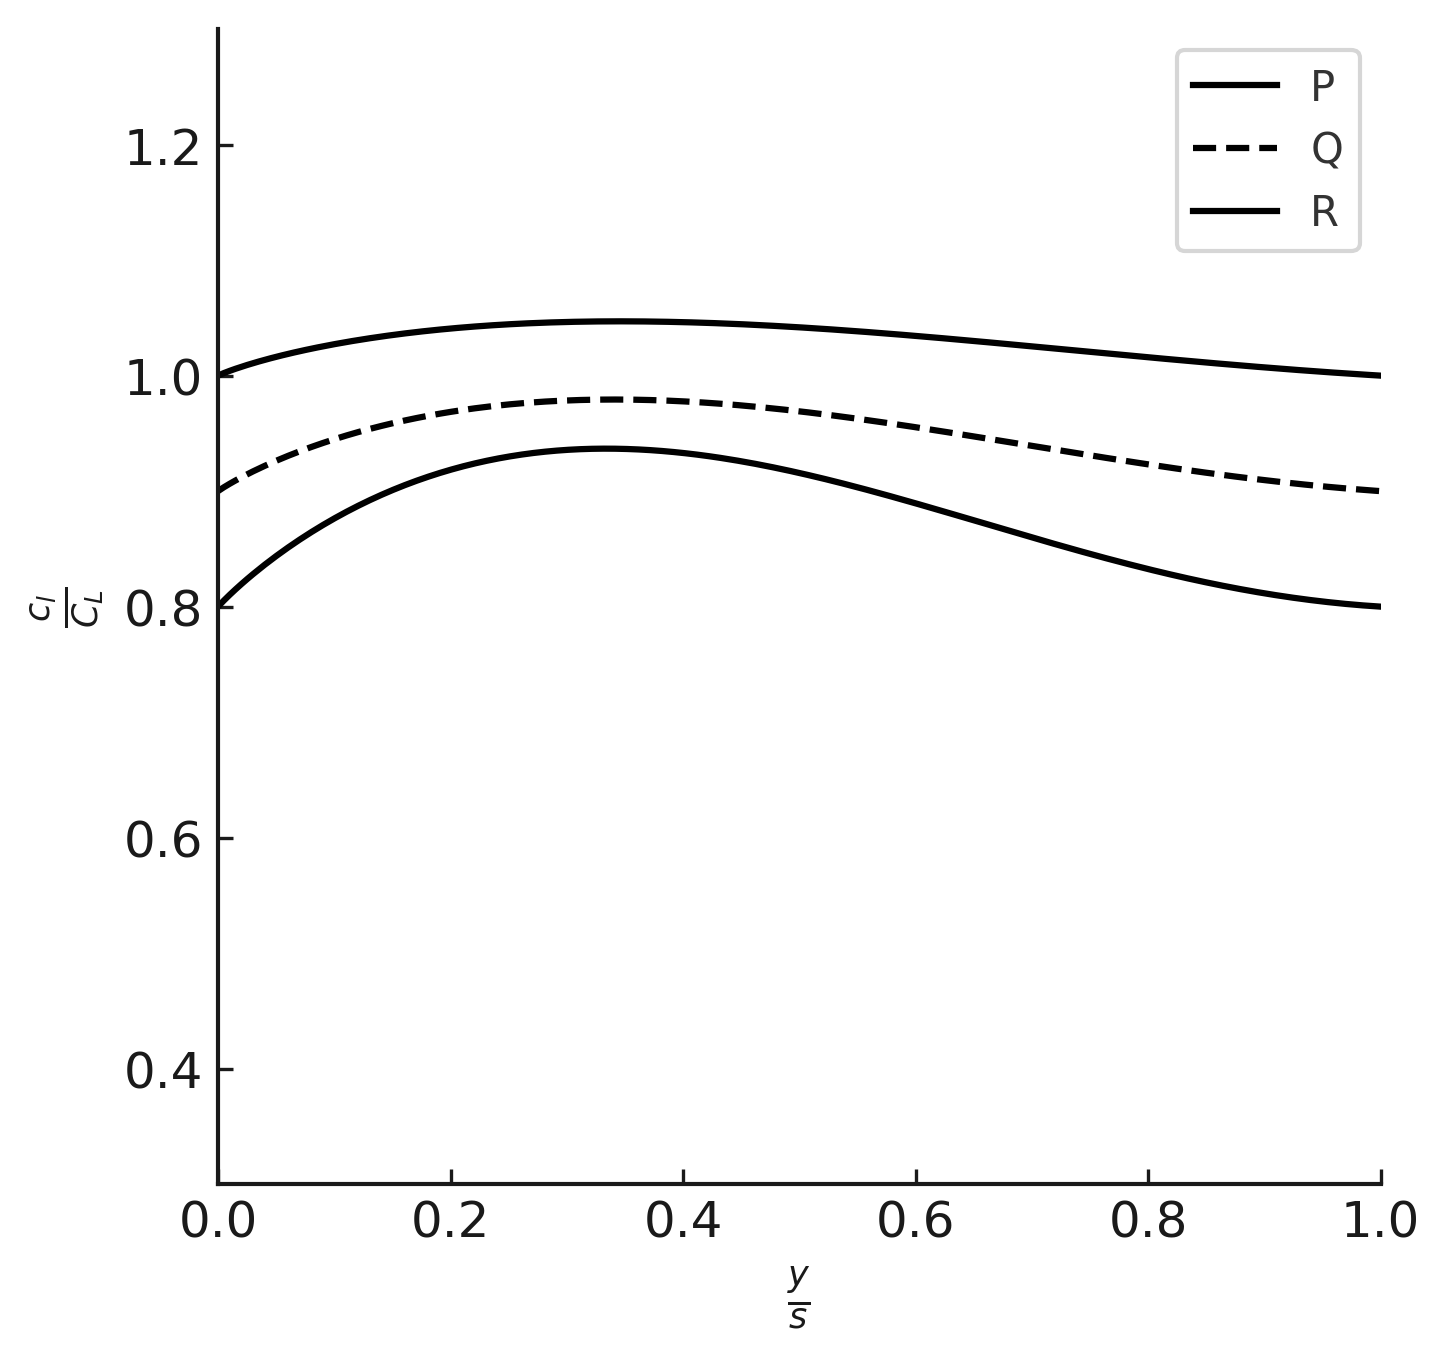
\includegraphics[width=0.5\columnwidth]{figs/q68.png}
        \caption{}
        \label{fig:q68}
    \end{figure}
    In the above figure, $c_l$ refers to the section lift coefficient, $C_L$ refers to the lift coefficient of the wing, $y$ is the coordinate along the span and $s$ is the span of the wing. A designer prefers to use a wing for which the stall begins at the root. Which of the wings will he choose?
    \begin{multicols}{4}
    \begin{enumerate}
        \item P
        \item Q
        \item R
        \item None
    \end{enumerate}
    \end{multicols}
    

    \item $\mathrm{\lim_{x \to 0} \frac{\sin x}{e^4 x} =}$
    \begin{multicols}{4}
    \begin{enumerate}
        \item 10
        \item 0
        \item 1
        \item $\infty$
    \end{enumerate}
    \end{multicols}
    

    \item Let a dynamical system be described by the differential equation $2 \frac{dx}{dt} + \cos x = 0$. Which of the following differential equations describes this system in a close approximation sense for small perturbation about $x = \pi/4$?
    \begin{multicols}{2}
    \begin{enumerate}
        \item $2 \frac{dx}{dt} + \sin x = 0$
        \item $2 \frac{dx}{dt} - \frac{1}{\sqrt{2}} x = 0$
        \item $\frac{dx}{dt} + \cos x = 0$
        \item $\frac{dx}{dt} + x = 0$
    \end{enumerate}
    \end{multicols}
    
\begin{center}
    \textbf{Common Data Questions}
\end{center}


\textbf{Common Data for Questions 71, 72 \& 73}: An airplane designer wants to keep longitudinal static stability margin (SM) within $5\%$ to $15\%$ of mean aerodynamic chor(D) A wind tunnel test of the model showed that for $\bar{X}_{CG} = 0.3$, $\frac{d C_m}{d C_L} = -0.1$. Note that the distance from the wing leading edge to the center of the gravity ($X_{CG}$) has been non-dimensionalized by dividing it with mean aerodynamic chord, $\bar{c}$, such that $\bar{X}_{CG} = X_{CG} / \bar{c}$. Note also that the relation $\frac{d C_m}{d C_L} = -SM$ holds true for this airplane.

    \item The most forward location of the airplane center of gravity to fulfill designer's requirement on longitudinal static stability is
    \begin{multicols}{4}
    \begin{enumerate}
        \item $0.35 \bar{c}$
        \item $0.45 \bar{c}$
        \item $0.52 \bar{c}$
        \item $0.67 \bar{c}$
    \end{enumerate}
    \end{multicols}
    

    \item The most aft location of the airplane center of gravity to fulfill designer's requirement on longitudinal static stability is
    \begin{multicols}{4}
    \begin{enumerate}
        \item $0.35 \bar{c}$
        \item $0.45 \bar{c}$
        \item $0.52 \bar{c}$
        \item $0.67 \bar{c}$
    \end{enumerate}
    \end{multicols}
    

    \item The center of gravity location to have $\frac{d \delta e}{d C_L} = 0$ is
    \begin{multicols}{4}
    \begin{enumerate}
        \item $0.35 \bar{c}$
        \item $0.45 \bar{c}$
        \item $0.5 \bar{c}$
        \item $0.4 \bar{c}$
    \end{enumerate}
    \end{multicols}
    
\end{enumerate}

\textbf{Common Data for Questions 74 \& 75}: Consider the spring mass system shown in the figure below. This system has two degrees of freedom representing the motions of the two masses.

\begin{figure}[H]
    \centering
    \usetikzlibrary{decorations.pathmorphing}

% Define spring style
\tikzset{
    spring/.style={
        decorate,
        decoration={
            coil,
            aspect=0.4,
            segment length=3mm,
            amplitude=3mm
        }
    },
    damper/.style={
        thick
    }
}

\begin{document}
\begin{tikzpicture}[thick]

% Left wall
\draw (-2,0.5) -- (-2,-0.5);

% First spring
\draw[spring] (-2,0) -- (-1,0);

% First mass (m)
\draw[fill=white] (-1,-0.5) rectangle (0.5,0.5);
\node at (-0.25,0) {$m$};
\draw (-0.25,0.6) [->] -- ++(0.6,0) node[right] {$x_1$};

% Middle spring
\draw[spring] (0.5,0) -- (1.5,0);

% Second mass (3m)
\draw[fill=white] (1.5,-0.5) rectangle (3,0.5);
\node at (2.25,0) {$3m$};
\draw (2.25,0.6) [->] -- ++(0.6,0) node[right] {$x_2$};

% Right spring
\draw[spring] (3,0) -- (4,0);

% Right wall
\draw (4,0.5) -- (4,-0.5);

% Labels for springs
\node at (-1.5,0.5) {$k$};
\node at (1,0.5) {$k$};
\node at (3.5,0.5) {$k$};

\end{tikzpicture}
\end{document}

    \caption{}
    \label{fig:q74 75}
\end{figure}

\begin{enumerate}
    \setcounter{enumi}{73}
    \item The system shows the following type of coordinate coupling
    \begin{enumerate}
        \item Static coupling
        \item Dynamic coupling
        \item Static and dynamic coupling
        \item No coupling
    \end{enumerate}

    \item The two natural frequencies of the system are given as
    \begin{multicols}{2}
    \begin{enumerate}
        \item $\sqrt{\frac{4 \pm \sqrt{5} k}{3 m}}$
        \item $\sqrt{\frac{4 \pm \sqrt{3} k}{3 m}}$
        \item $\sqrt{\frac{4 \pm \sqrt{7} k}{3 m}}$
        \item $\sqrt{\frac{4 \pm \sqrt{11} k}{3 m}}$
    \end{enumerate}
    \end{multicols}
    
\end{enumerate}

\begin{center}
    \textbf{Linked Answer Questions: Q. 76 to Q. 85 carry two marks each}
\end{center}


\textbf{Statement for Linked Answer Questions 76 \& 77}: For a piston propeller airplane weighing $20000 \, \mathrm{N}$, the flight testing at $5 \, \mathrm{km}$ pressure altitude in standard atmosphere gave the variation of power required versus true air speed as shown in figure below. The student forgot to label the air speed axis. The maximum climb rate at sea level was calculated to be $3.65 \, \mathrm{m/s}$ at air density $1.225 \, \mathrm{kg/m^3}$ and $0.815 \, \mathrm{kg/m^3}$, respectively.

\begin{figure}[H]
    \centering
    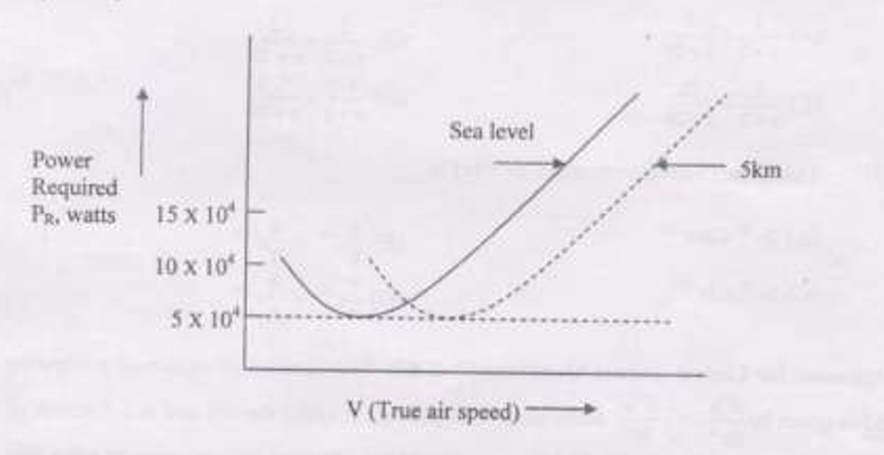
\includegraphics[width=0.5\columnwidth]{figs/q76 77.png}
    \caption*{}
    \label{fig:q76 77}
\end{figure}

\begin{enumerate}
    \setcounter{enumi}{75}
    \item The maximum rate of climb achievable by this airplane at $5 \, \mathrm{km}$ altitude will be
    \begin{multicols}{4}
    \begin{enumerate}
        \item $1.65\ m/s$
        \item $0.51\ m/s$
        \item $1.43\ m/s$
        \item $3.65\ m/s$
    \end{enumerate}
    \end{multicols}
    

    \item If during the maximum rate of climb at $5 \, \mathrm{km}$ altitude, the airplane was flying at an angle of attack of 4 degrees and attitude (pitch) angle of 5 degrees, what was equivalent airspeed of the airplane?
    \begin{multicols}{4}
    \begin{enumerate}
        \item $40.2\ m/s$
        \item $63.7\ m/s$
        \item $130.3\ m/s$
        \item $20.2\ m/s$
    \end{enumerate}
    \end{multicols}
    
\end{enumerate}

\textbf{Statement for Linked Answer Questions 78 \& 79}: A model wing of rectangular planform has a chord of $0.2 \, \mathrm{m}$ and a span of $1.2 \, \mathrm{m}$. It has a symmetric airfoil section whose lift curve slope is 0.1 per degree. When this wing is mounted at 8 degrees angle of attack in a freestream of $20 \, \mathrm{m/s}$ it is found to develop $35.3 \, \mathrm{N}$ lift when the density of air is $1.225 \, \mathrm{kg/m^3}$.

\begin{enumerate}
    \setcounter{enumi}{77}
    \item The lift curve slope of this wing is
    \begin{multicols}{4}
    \begin{enumerate}
        \item 0.10 per deg
        \item 0.092 per deg
        \item 0.075 per deg
        \item 0.050 per deg
    \end{enumerate}
    \end{multicols}
    

    \item The span efficiency factor of this wing is
    \begin{multicols}{4}
    \begin{enumerate}
        \item 1.0
        \item 0.91
        \item 0.75
        \item 0.63
    \end{enumerate}
    \end{multicols}
    
\end{enumerate}

\textbf{Statement for Linked Answer Questions 80 \& 81}:
Let $F(s) = \frac{(s + 10)}{(s +2)(s + 20)}$

\begin{enumerate}
    \setcounter{enumi}{79}
    \item The partial fraction expansion of $F(s)$ is
    \begin{multicols}{2}
    \begin{enumerate}
        \item $\frac{1}{s + 2} + \frac{1}{s + 20}$
        \item $\frac{5}{s + 2} + \frac{2}{s + 20}$
        \item $\frac{2}{s + 2} + \frac{20}{s + 20}$
        \item $\frac{4/9}{s + 2} + \frac{5/9}{s + 20}$
    \end{enumerate}
    \end{multicols}
    

    \item The inverse Laplace transform of $F(s)$ is
    \begin{multicols}{2}
    \begin{enumerate}
        \item $2e^{-34} + 20e^{-34}$
        \item $\frac{4}{9}e^{-34} + \frac{5}{9}e^{-34}$
        \item $5e^{-34} + 2e^{-34}$
        \item $\frac{9}{4}e^{-34} + \frac{9}{5}e^{-34}$
    \end{enumerate}
    \end{multicols}
    
\end{enumerate}

\textbf{Statement for Linked Answer Questions 82 \& 83}: The equation of motion of a vibrating rod is given by $\frac{\partial^2 u}{\partial t^2} = c^2 \frac{\partial^2 u}{\partial x^2}$. Here $u$ is the displacement along the rod and is a function of both position $x$ and time $t$. To find the response of the vibrating rod, we need to solve this equation using boundary conditions and initial conditions.

\begin{enumerate}
    \setcounter{enumi}{81}
    \item The boundary conditions needed for a rod fixed at the root ($x=0$) and free at the tip ($x=l$) are
    \begin{multicols}{2}
    \begin{enumerate}
        \item $u(x=0) = 0, \frac{\partial u}{\partial x}(x=l) = 0$
        \item $u(x=l) = 0, \frac{\partial u}{\partial x}(x=l) = 0$
        \item $u(x=0) = 0, u(x=l) = 0$
        \item $\frac{\partial u}{\partial x}(x=0) = 0, \frac{\partial u}{\partial x}(x=l) = 0$
    \end{enumerate}
    \end{multicols}
    

    \item The natural frequencies $\omega$ of the fixed-free rod can then be obtained using
    \begin{multicols}{4}
    \begin{enumerate}
        \item $\cos \left( \frac{\omega l}{c} \right) = 0$
        \item $\sin \left( \frac{\omega l}{c} \right) = 0$
        \item $\cos \left( \frac{\omega c}{l} \right) = 0$
        \item $\cos \left( \frac{\omega}{c} \right) = 0$
    \end{enumerate}
    \end{multicols}
    
\end{enumerate}

\textbf{Statement for Linked Answer Questions 84 \& 85}: Air enters the compressor of a gas turbine engine with velocity $127 \, \mathrm{m/s}$, density $1.2 \, \mathrm{kg/m^3}$ and stagnation pressure $0.9 \, \mathrm{MPa}$. Air exits the compressor with velocity $139 \, \mathrm{m/s}$ and stagnation pressure $3.15 \, \mathrm{MPa}$. Assume that the ratio of specific heats is constant and equal to 1.4.

\begin{enumerate}
    \setcounter{enumi}{83}
    \item The compressor pressure ratio is
    \begin{multicols}{4}
    \begin{enumerate}
        \item 0.22
        \item 0.28
        \item 3.50
        \item 3.90
    \end{enumerate}
    \end{multicols}
    

    \item If the polytropic efficiency of the compressor is 0.89, then the isentropic efficiency of the compressor is
    \begin{multicols}{4}
    \begin{enumerate}
        \item 0.613
        \item 0.869
        \item 0.89
        \item 0.98
    \end{enumerate}
    \end{multicols}
\end{enumerate}

\begin{center}
{\Large \textbf{END OF THE QUESTION PAPER}}
\end{center}

\end{document}